%%%%%%%%%%%%%%%%%%%%%%%%%%%%%%%%%%%%%%%%%%%%%%%%%%%%%%%%%%%%%%%%%%%%%%%%%%%%%%%%%%%%
The Coronavirus Disease 2019 (COVID-19) pandemic indicates how great of a need there is for accurate and fast modeling methods. In this thesis, I describe a model that incorporates the spatial spread of viruses and produces accurate simulations in a few seconds or minutes, so that the model can be used to study viruses in a more accurate way. 

\section{Basic Virology}

Viruses are microscopic parasites, generally much smaller than bacteria, that lack the capacity to thrive and reproduce outside of a host body. A virus is composed of a nucleic acid genome and a protein capsid that covers the genome. As seen in figure \ref{fig:Virus_Replication}, the life cycle of a virus begins with the virus attaching to or being absorbed by the host cell. Once the virus genome enters into a cell, the genome moves to the ribosomes, where the genome is replicated. After the genome is replicated, new virus can be assembled and released from the host cell, allowing the virus to continue spreading throughout the host cells \citep{openstax_microbiology_2016}.

\begin{figure}[h]
    \centering
    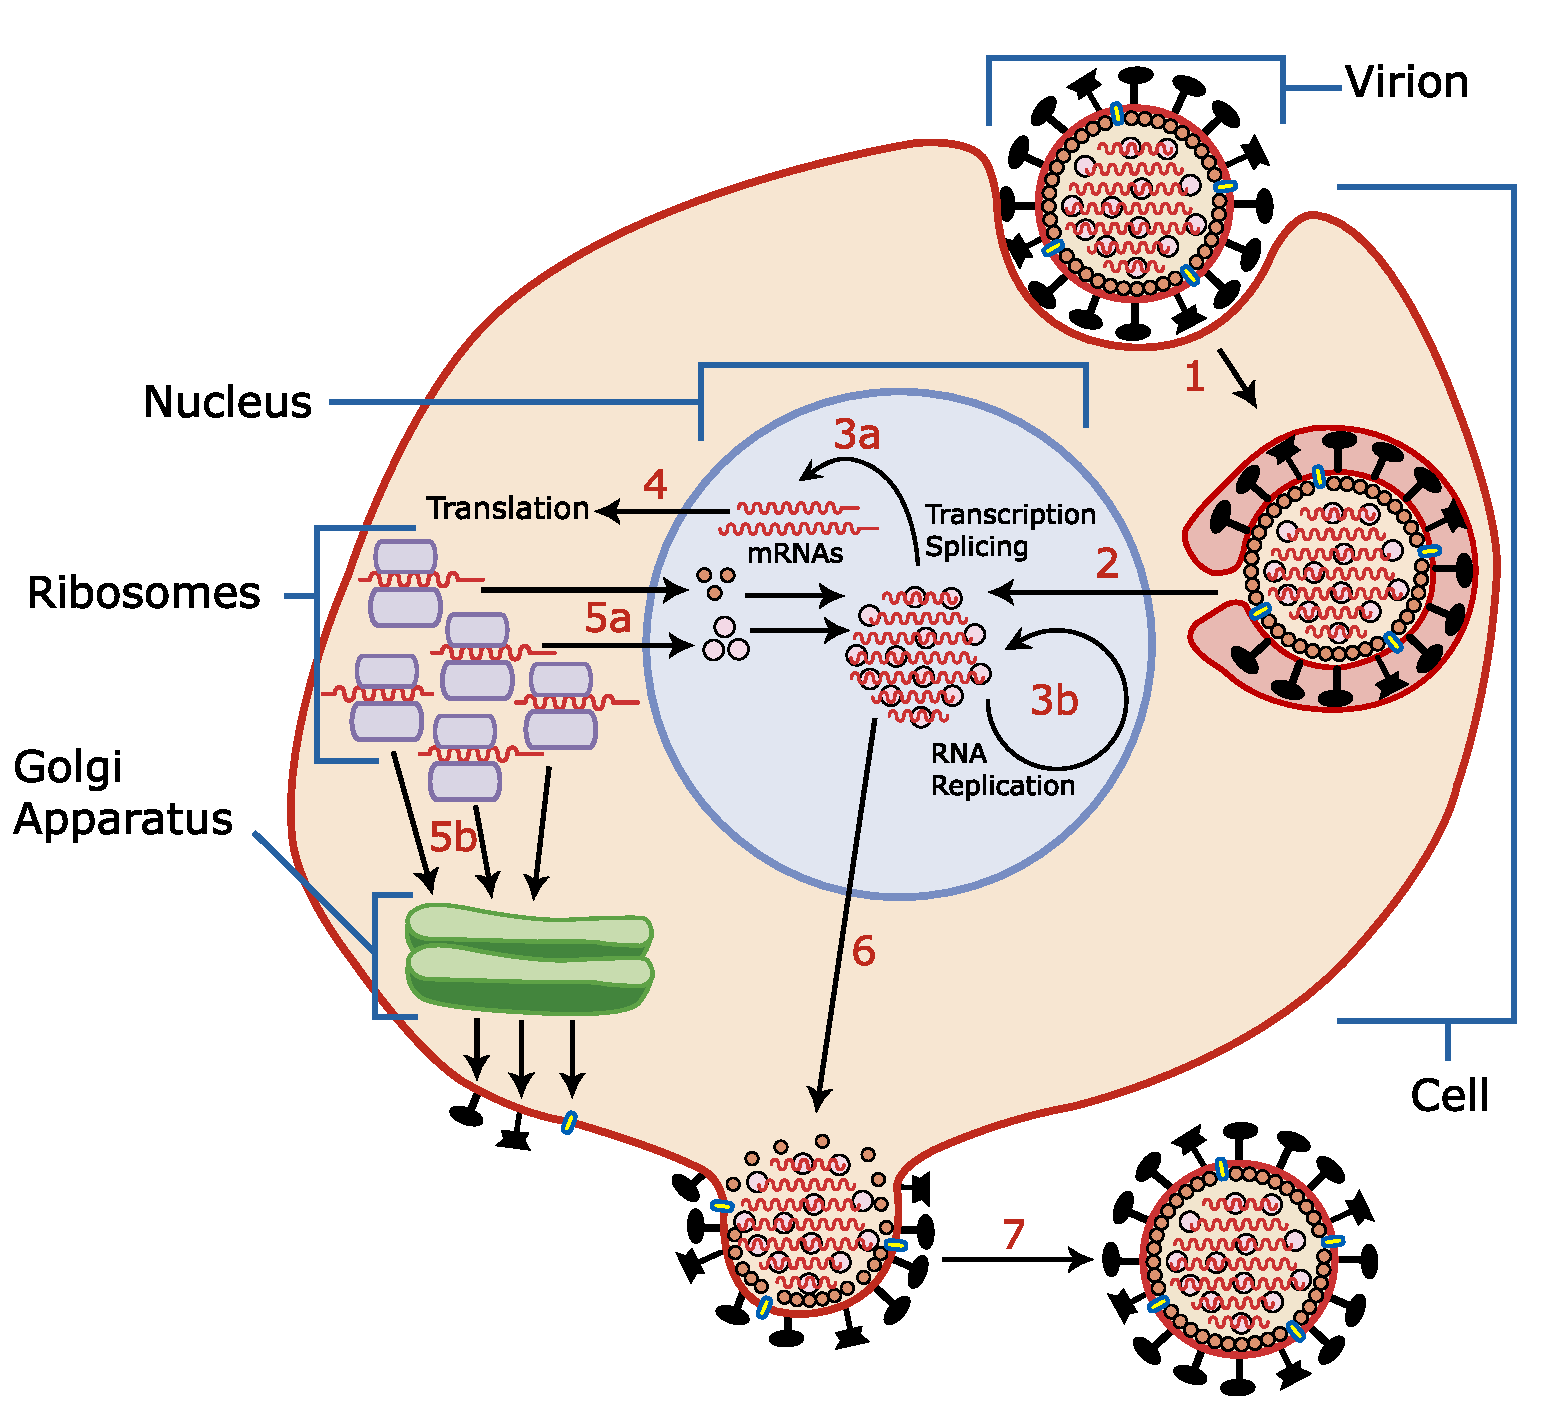
\includegraphics[width=0.6\linewidth]{Figures/Virus_Replication_large.pdf}
    \caption{The life cycle of a virus begins with a virion (virus particle) being absorbed by the cell. Once the virion enters into a cell the virus genome is released. The genome moves to the ribosomes, where the genome is replicated. With the replicated genome, new virus can be assembled by the golgi apparatus and then released from the cell.}
    \label{fig:Virus_Replication}
\end{figure}

Some viruses cause illnesses and the spread of a few has been severe enough to cause global pandemics (global outbreaks). Recent examples are the current 2019-2021 Covid-19 pandemic, the 2014 Ebola pandemic, and the 2009 Swine Flu pandemic. Other viruses are endemic (regional outbreak) or occur seasonally (yearly outbreaks); for example, influenza (flu) is know for it's spread each year in the United States. In total, the Centers for Disease Control and Prevention estimates that in the United States up to 42.9 million people were sick during the 2018-2019 flu season, 647,000 people were hospitalized, and 61,200 died. \citep{xu_update_2019}

In order to understand viruses, assays are performed. An assay is an experiment for assessing or measuring characteristics of a substance. There are two ways the assays are carried out, \emph{in vitro} or \emph{in vivo}. \emph{In vitro} assays are assays that are performed outside of a living organism. In virology, the plaque assay is the type of \emph{in vitro} assay that is most widely used for determining viral titer \citep{pankaj_virus_2021}.  These assays are often performed on a monolayer of cells in petri dishes or multi-well plates with a small number of wells. The dishes and plates are a type of adherent culture where the cells are grown on a nutritious substrate. The cells are grown to cover the entire surface (the point of confluence), at this point the cells tend to push on each other and distort the shape of each cell membrane \citep{bruckner_importance_2018}. Each dish/well has on the order of \numrange[range-phrase = --]{e5}{e6} cells grown on it's surface \citep{Number_of_cells_in_a_dish}. When the assay is performed, virus is placed in a dish/well of healthy cells. Any virus that causes damage to the cells in the dish/well can be studied. This damage is called a plaque and is roughly circular in shape. During the assay, formation of plaques and the concentration of virus are monitored. It is assumed that each plaque formed is caused by one virus particle. Because of this assumption, the viral concentration is often recorded as plaque forming units per milliliter (PFU/mL). 

\emph{In vivo} assays are assays that are performed in a multi-cellular living organism. Any virus that will infect the target animal can be studied. When the assay is performed, virus is introduced to the target animal through a nasal spray or injection. Then during the assay any visible symptoms and viral concentration are monitored.% by a nasal swab, blood test, or (as seen with mice) extraction from the lungs once the animal is sacrificed.

%%%%%%%%%%%%%%%%%%%%%%%%%%%%%%%%%%%%%%%%%%%%%%%%%%%%%%%%%%%%%%%%%%%%%%%%%%%%%%%%%%
\section{Modeling of assays}

In recent years, the field of virology has started using agent-based models to study the spread of viruses during \emph{in vitro} viral infection assays \citep{beauchemin_simple_2005,alvarado_cellular-level_2018,wodarz_laws_2014,tong_development_2015,whitman20,goyal16,itakura10,wasik14} in an effort to study the spatiality of viral spread. The agent-based model framework is appealing to virus modelers because it allows for the individual tracking of how cells, as agents, interact with the virus, and has the potential to replicate \emph{in vitro} and eventually \emph{in vivo} viral infections. 

Agent-based (individual-based or micro-simulation) models have been around since 1970 with the introduction of ``Conway's Game of Life'' \citep{gardner70}. These models have been utilized in many different fields from physics to the study of fish (ichthyology) \citep{owusu20} and continue to be popularized for different applications by software like Netlogo \citep{nogare20,chiacchio14}. The models consist of a collection of agents whose behavior is determined by mathematical or computational rules. The agents of the system can move freely \citep{beauchemin07} or be fixed in a grid or lattice \citep{beauchemin_simple_2005} for varying applications, but either configuration allows for tracking of spatially emergent patterns. To date, unfortunately, the implementation of agent-based models for simulating viral infections has had two issues: speed and size.

Agent-based models are notorious for being computationally intensive and taking long amounts of time to run simulations. This point has been commented on in a review of spatiotemporal models of viral infection \citep{gallagher_causes_2018} and the feasibility of agent-based models for viral infection research has been talked about as a goal that is to come with increasing computational advancements \citep{bauer_agent-based_2009}. Previous research has addressed this lack of computing power issue by reducing the number of agents modeled and therefore reducing the number of computations required for a simulation. The number of agents published is at minimum an order of magnitude lower than the number of target cells used in the corresponding experimental data. Beauchemin et al.\ \citep{beauchemin_simple_2005} simulated \num{1.232e5} agents, while the experiment they were attempting to replicate was performed in 6 well-plates and had $\sim$\num{1.2e6} cells per well. Alvarado et al.\ \citep{alvarado_cellular-level_2018} simulated \num{4.0e4} agents when trying to replicate experiments also performed in 6 well-plates. Wodarz et al.\ \citep{wodarz_laws_2014} simulated \num{2.0e4} agents, while the experiment they were replicating was performed in 24 well-plates and had $\sim$\num{2.4e5} cells per well. Tong et al.\ \citep{tong_development_2015} simulated \num{6.0e5} agents in an effort to simulate mice lungs, which have $\sim$\num{e9} cells. These smaller simulations are more affected by boundary interactions, which can result in model dynamics that don't faithfully reproduce the infection. Having an in-host model that can produce accurate simulations in a timely manner not only allows for the prediction of patient infection, but also can be used to flush out potential causes of varying symptoms in patients. 

%%%%%%%%%%%%%%%%%%%%%%%%%%%%%%%%%%%%%%%%%%%%%%%%%%%%%%%%%%%%%%%%%%%%%%%%%%%%%%%%%%
\section{Exigence}
While it might be feasible to wait long periods of time to run accurate simulations for endemic or recurrent seasonal viruses, recent events of the COVID-19 pandemic indicate how great a need there is for accurate and fast modeling methods. Epidemiological population-level modeling tools that include both ordinary differential equation models \citep{li20,ngonghala20} and agent-based models \citep{ying21,sneppen21,kano21} were immediately deployed to help predict how the new virus would spread around the world and how different interventions could help stem the spread. At the within-host level, the primary modeling tool was limited to simple ordinary differential equation models \citep{goncalves20,wang20model,hernandez20,dogra20} that lack the ability to reproduce the spatial heterogeneity of real viral infections. Fast and accurate in-host models could be helpful in assessing the potential of re-purposed drugs \citep{czuppon21,goncalves20,dodds20}, finding indicators of disease severity or mortality \citep{neant21}, and assessing the effectiveness of testing \citep{ejima21}. A community-driven agent-based model incorporating many realistic biological responses was quickly developed for Severe Acute Respiratory Syndrome Coronavirus 2 (SARS-CoV-2) \citep{getz21}, but is only currently simulating a few thousand agents and is expected to need high-performance computing or cloud resources to parameterize the model. Thus, there is a need to develop modeling and simulation tools for accurately predicting in-host viral dynamics that can be quickly deployed to help combat the next pandemic.

%%%%%%%%%%%%%%%%%%%%%%%%%%%%%%%%%%%%%%%%%%%%%%%%%%%%%%%%%%%%%%%%%%%%%%%%%%%%%%%%%
\section{Scope}

In this work, the testing, validation, and application of a hybrid agent-based model and partial differential equation model implemented on graphics processing units is presented. The work here begins with the methods where the four attributes of the model: (1) the agent-based model of the cells, (2) the partial differential equation of the virus, (3) the cell-free transmission mode of viruses, and (4) fitting of the model to data, are explained.  Then, the results of model implementation with parallel programming, convergence testing, and simulation speed improvement are presented. Finally, I show that the model can reproduce experiments by fitting the model to an \emph{in vitro} influenza virus experiment and an \emph{in vitro} SARS-Cov-2 experiment. This work shows how an agent-based and partial differential equation hybrid model of in-host infections is tested for numerical convergence, is applied to experimental data for parameter extraction, and produces simulations within seconds to minutes for timely application. 




